%!TEX root = report.tex
\newpage
\section{Experimental Setup}

% Camera
\subsection{Camera Setup}

\paragraph{Hardware} The camera is made of a Raspberry Pi 2 Model B with the corresponding Raspi-Camera module. The OS loaded to the camera is the common Raspian WHEEZY system with 3 scripts running on startup in the background. The camera connected is the Raspi-Camera module.
The camera has the following key parameters: \cite{RaspiDoc}
\begin{itemize}
    \item Pixel Count: 2592 x 1944
    \item Pixel size 1.4 x 1.4 $\mu m$
    \item Focal width and length: f=3.6mm
\end{itemize}

\begin{figure}[H]
    \centering
    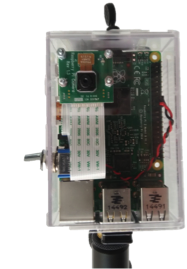
\includegraphics[width=0.3\linewidth]{files/RaspiCam.png}
    \caption{Raspberry Pi with camera module used for visual localization}
    \label{fig:camera}
\end{figure}


\paragraph{Webcam setup} In order to connect to the LAN on startup, a few lines need to be added in $/etc/network/interfaces$: 

\begin{center}
\begin{minipage}{0.9\linewidth}
\begin{lstlisting}[caption=$/etc/network/interfaces$, label=interfaces, frame=none]
auto lo
iface lo inet loopback

iface eth0 inet static
address 172.16.156.138
netmask 255.255.255.0
gateway 172.16.156.1

auto wlan0
allow-hotplug wlan0
iface wlan0 inet static
address 172.16.156.139
netmask 255.255.255.0
gateway 172.16.156.1
wireless-essid korebot
\end{lstlisting}
\end{minipage}
\end{center}

The camera module comes with an own library with modules for taking single images ($raspistill$) or videos ($raspivid$).
The following lines of code are added in a file $\sim\hspace{-0.5em}/start\_camera.sh$ in order to take pictures at regular intervals and save them to $/tmp/stream$. This is where they will be found by the $mjpg_streamer$ module which sends the images to the corresponding server.

\begin{center}
\begin{minipage}{0.9\linewidth}
\begin{lstlisting}[caption=$\sim\hspace{-0.5em}/start\_camera.sh$, label=startcamera, frame=none]
#!/bin/bash
echo "Start camera stream"

sudo mkdir -p /tmp/stream
sudo chmod 777 /tmp/stream
raspistill -w 1280 -h 720 -q 50 -ex backlight -mm backlit -o /tmp/stream/pic.jpg -tl 100 -t 2147483647 &
LD_LIBRARY_PATH=/usr/local/lib mjpg_streamer -i "input_file.so -f /tmp/stream -n pic.jpg" -o "output_http.so -w /usr/local/www"
\end{lstlisting}
\end{minipage}
\end{center}

Line 6 tells the camera to take a picture of resolution $w \times h = 1280 \times 720$ of quality 50\% (100\% would mean no compression at all), at a time interval of $tl = 100ms$ until the time $t = 2147483647ms = 24 \text{d} 19 \text{h}$ is reached, which is the maximum for a 32-bit signed integer.
Other parameters like the exposure, set to backligh, and the metering mode can be set. 
With these settings, the resulting picture size is of about $N_{pic}=455kB$, to compared with a size of around $N_{pic}=533$ for 100\% quality. The way the image compression is implemented, there is nearly no difference in size down to a quality of around 20\% and the loss in quality is negligible (see Figure \ref{fig:quality}).
This size is just too big for the chosen Router with capacity of about 150 Mbps, considering that in the worst case, the images from the 4 cameras are required simultaneously. Therefore the quality is set down to 10, which is a good trade off between image quality (see Figure \ref{fig:quality}) and size (100 kB). Indeed, this quality is said to be equivalent to a quality of around 85\% for most applications by Raspberry Pi users. %TODO add citation?
In addition to that, the thumbnail, which is a bitmap that also takes up unnecessary storage space, is deleted and a final image size of 80 kB is obtained. This is an acceptable size since we have:

\begin{figure}[htb]
    \centering
    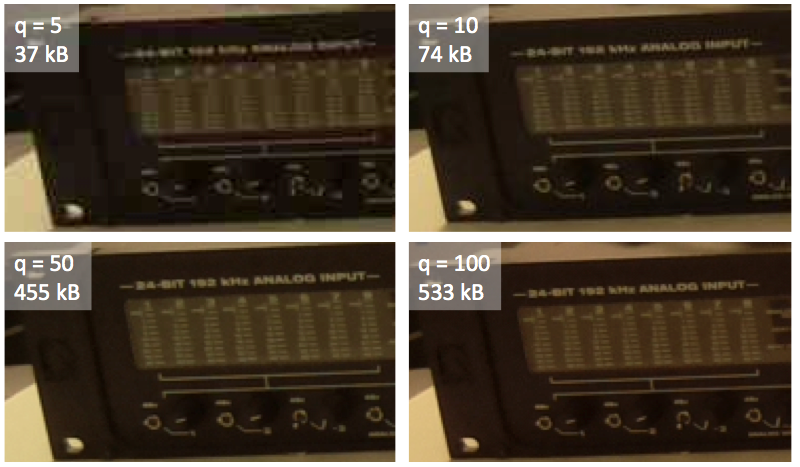
\includegraphics[width=.8\linewidth]{files/quality.png}
    \caption{Quality vs. image size considerations}
    \label{fig:quality}
\end{figure}

\begin{equation}
    S_{network} = 150 \text{ Mbps} = 18.75 \text{ MB/s} \geq \frac{N_{pic}}{tl}  = \frac{80/1024 MB}{0.1\text{s}}= 0.78 \text{ MB/s}
\end{equation}

This leads to a reasonable security margin, which is desirbale since the declared maximum capacity is largely overestimated in comparison with practical measurements, indicating a capacity of only 1.5-1.7 MB/s.

Line 7 starts the mjpg streamer from where the picture has been stored and serves them on a webpage. The mjpg streamer is a Linux-UVC streaming application which streams JPGs from wecams, filesystems or other input plugins via as M-JPEG, which is a common video compression format, via HTTP to webbrowsers.

\paragraph{Button}

A button is added to the camera such that it can be restarted or turned off without logging into the camera. This allows the Raspberry to be turned off correctly even when the network has not be set up properly or the ethernet is not working.
The button is a pull-down resistor, thus the signal at the output goes from 0 to 1 when the button is pressed. An interrupt is triggered when the button is pressed in which it counts during 6 seconds weather the button is pressed or not at a rate of 1s. For robustness, a total of 3 signals is sufficient for the system to shut down. If less than 3 signals are registered during the 6 seconds, the system reboots. 

\begin{center}
\begin{minipage}{0.9\linewidth}
\begin{lstlisting}[caption=$\sim\hspace{-0.5em}/switchoff.sh$, label=switchoff, language=Python, frame=none]
#-*- coding: utf8 -*-
import RPi.GPIO as GPIO
import os
import time
#set up GPIO using BCM numbering
GPIO.setmode(GPIO.BCM)
GPIO.setup(10,GPIO.IN, pull_up_down=GPIO.PUD_DOWN)

#function called on pin interrupt
def button_triggered(channel):
        counter = 0
        counter_on = 0
        while (counter <= 6):
                time.sleep(1)
                counter+=1
                if (GPIO.input(10)):
                        counter_on+=1
                if (counter_on >= 3):
                        break

        if (counter_on >= 3):
                print("switchoff.py: Raspberry shutting down now")
                os.system("sudo halt")
        elif (counter_on < 3):
                print("switchoff.py: Rapsberry is going to reboot now")
                os.system("sudo reboot")
#setup pin interrupt
GPIO.add_event_detect(10,GPIO.RISING,callback=button_triggered,bouncetime=300)

#wait forever
while True:
        time.sleep(0.001)

GPIO.cleanup()
\end{lstlisting}
\end{minipage}
\end{center}


Both scripts above need to be started on startup of the camera. Therefore, the following lines are put in the file /etc/rc.local:
\begin{center}
\begin{minipage}{0.9\linewidth}
\begin{lstlisting}[caption=$/etc/rc.local$, label=local, frame=none]
#Auto start camera
sudo /home/pi/start_camera.sh &
#Auto start shutdown
sudo python /home/pi/switchoff.py &
\end{lstlisting}
\end{minipage}
\end{center}

\newpage
\subsection{Audio Setup}
The tools used for the audio recording are two wireless audio transmitters with their corresponding 
receivers (see Figure \ref{fig:audio}). The transmitters are connected to microphones placed in the Robot ears and the receivers are connected to two channels of the soundcard.

\begin{figure}[H]
    \centering
    \begin{subfigure}{0.25\linewidth}
        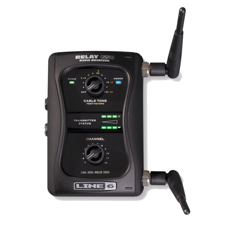
\includegraphics[width=\linewidth]{files/Receiver.png}
    \end{subfigure}
    \begin{subfigure}{0.25\linewidth}
        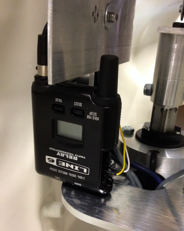
\includegraphics[width=\linewidth]{files/Transmitter.png}
    \end{subfigure}
    \caption{Wireless audio receiver (left) and transmitter (right)}
    \label{fig:audio}
\end{figure}

A conventional speaker is fixed on the robot and operated via the same soundcard. 

\subsection{Robot}

\begin{figure}[H]
    \centering
    \begin{subfigure}{0.3\linewidth}
        \centering
        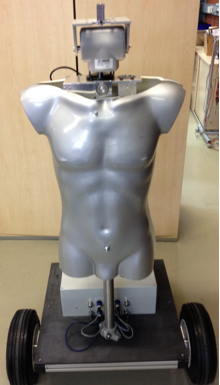
\includegraphics[height=0.3\textheight]{files/Robot.png}
        \caption{at rest}
    \end{subfigure}
    \begin{subfigure}{0.3\linewidth}
        \centering
        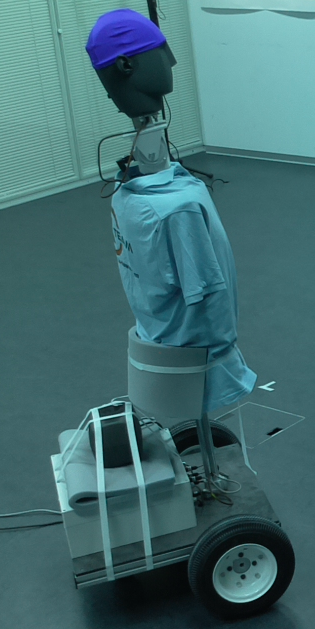
\includegraphics[height=0.3\textheight]{files/Robot2.png}
        \caption{in action - side view}
    \end{subfigure}
    \begin{subfigure}{0.3\linewidth}
        \centering
        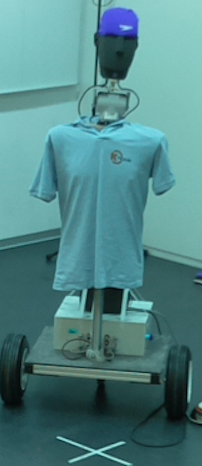
\includegraphics[height=0.3\textheight]{files/Robot3.png}
        \caption{in action - front view}
    \end{subfigure}
    \caption{Robot designed by Gigatec S.A. for Echo SLAM}
\label{fig:robot}
\end{figure}

The robot used for these experiments was designed by Gigatec S.A. It is shown in Figure \ref{fig:robot}.
It comes with already implemented code for its movement control. 
Two wheels can be actuated for displacement (see \par \ref{sec:movement}) and the acoustic head can be rolled, pitched and yawed independently. 
For the present setup, the head always stays in the standard (straight) position.

For good autonomy, the robot is actuated via a socket interface and the AF\_INET protocol. All commands are sent via a simple python script. For manual operation of the robot, some commands can also be sent via ssh.


%picture quality and compression:
%\url{www.raspberrypi.org/forum/viewtopic.php?f=43&t=73174&p=527300#p527300}
%wget:
%\url{https://www.maketecheasier.com/test-internet-connection-speed-from-terminal/}
%speedtest:
%http://www.speedtest.net/
